\section{MUSIC-algoritmin simulointi}
Tässä kandidaattityössä käytettiin Matlab-ohjelmaa simuloimaan MUSIC-algoritmia ja sen eri versioita. Simulaatioita tehtiin yksinkertaisella pallomallilla sekä todellisten aivojen mallilla, jotka muodostettiin MRI-kuvantamisen avulla. Apukoodit simulointiin on saatu Jukka Sarvakselta sekä Matti Stenroosilta.

MUSIC-algoritmia voidaan testata yksinkertaisella pallomallilla. Tässä mallissa elektrodit ja lähdepisteet sijotetaan pallokuoren yläpäähän ja sitten projisoidaan stereograafisen projektion avulla tasoon.

Kuvissa \ref{fig:mfix} ja \ref{fig:mfree} on simuloitu MUSIC-algoritmia sekä kiinnitetyllä että vapaalla orientaatiolla. Simuloinneissa kolme lähdedipolia sijoitettiin aivokuorelle, jotka on merkitty punaisina renkaina ja topografia on muodostettu MUSIC-algoritmin avulla.

Kuvissa \ref{fig:RAPfix} ja \ref{fig:RAPfree} on simuloitu RAP-MUSIC- algoritmia kiinnitetyllä ja vapaalla orientaatiolla. Kuvissa musta rasti kuvaa paikannusfunktion maksimiarvon paikkaa ja löydetyt dipolit merkataan punaisella neliöllä.

Kuvista huomataan, että MUSIC vapaalla orientaatiolla saa aikaan suuria aktiivisuuden alueita, mikä vaikeuttaa lähteiden paikantamista.


\clearpage
\begin{figure}[h]
    \centering
    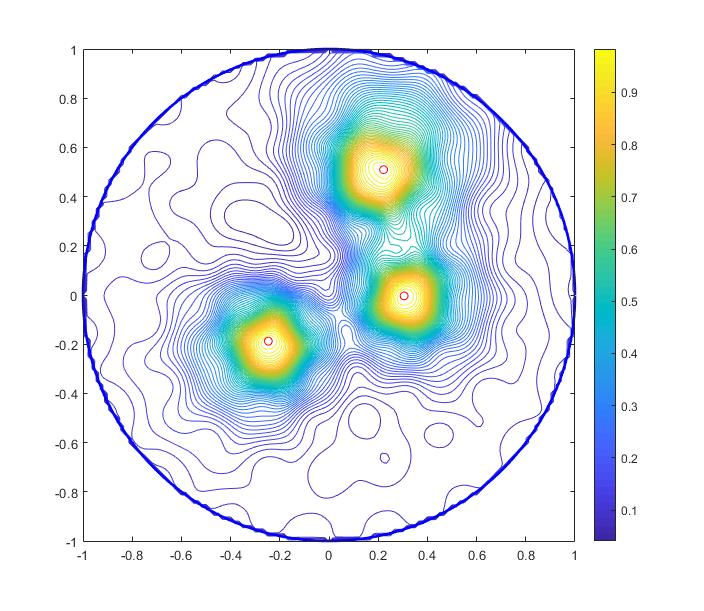
\includegraphics[scale=0.38]{mfix.jpg}
    \caption{MUSIC-algoritmin simulointi pallomallilla kiinnitetyllä orientaatiolla.}
    \label{fig:mfix}
\end{figure}

\begin{figure}[h]
    \centering
    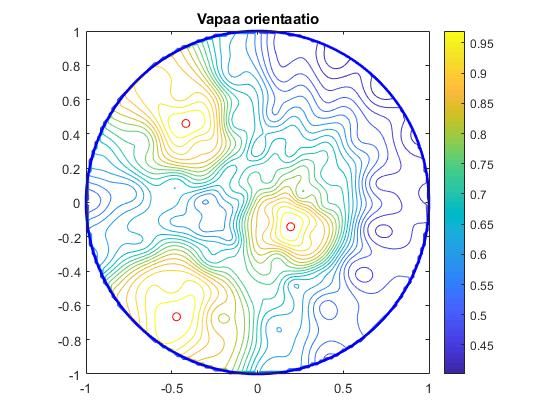
\includegraphics[scale=0.4]{mfree.jpg}
    \caption{MUSIC-algoritmin simulointi pallomallilla vapaalla orientaatiolla.}
    \label{fig:mfree}
\end{figure}

\clearpage

\begin{figure}[ht]
    \centering
    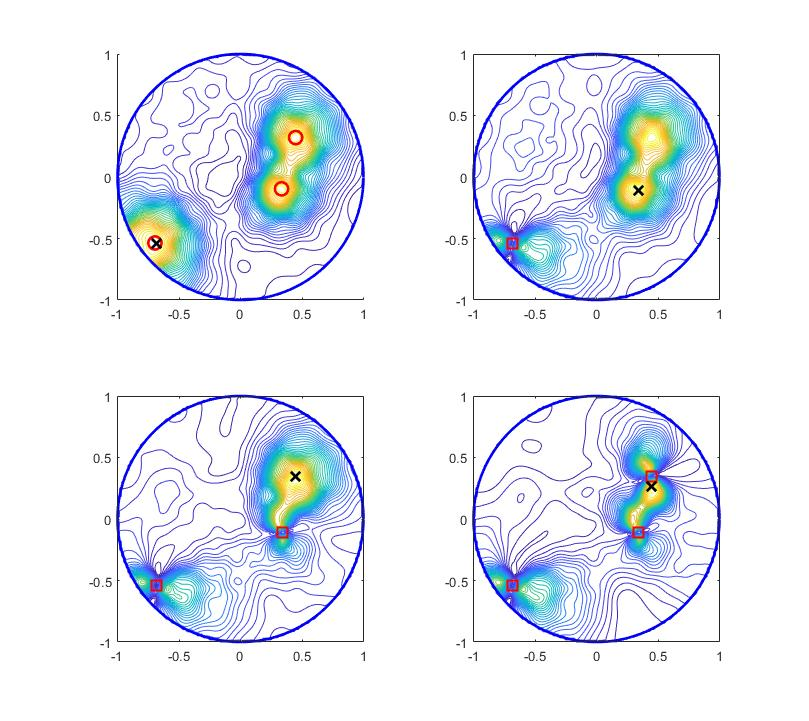
\includegraphics[width=\textwidth]{RAPfixed.jpg}
    \caption{RAP-MUSIC kiinnitetyllä orientaatiolla}
    \label{fig:RAPfix}
\end{figure}

\clearpage
\begin{figure}[ht]
    \centering
    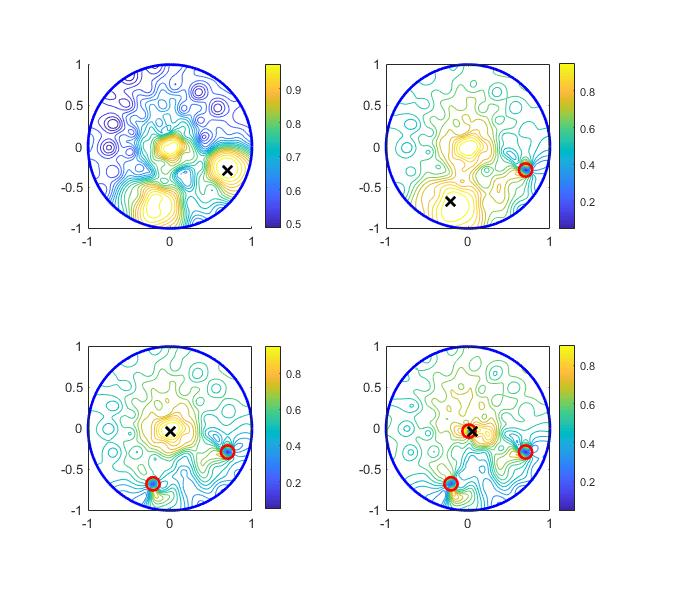
\includegraphics[width=\textwidth]{RAPfree.jpg}
    \caption{RAP-MUSIC vapaalla orientaatiolla}
    \label{fig:RAPfree}
\end{figure}